\graphicspath{{chapters/_resources/}}

\chapter{Genome instability and DNA damage response and repair}


\hypertarget{r-loops}{%
\section{R-loops}\label{r-loops}}

RNA is quickly displaced as soon as it emerges from Pol II; during transcription RNA-DNA hybrid structure is required, but it is \emph{transient}. It has been observed that RNA can re-hybridize with the template DNA forming \textbf{RNA:DNA hybrid} and \textbf{R-loop structures} (Figure \ref{fig:hybrid}). R-loop formation results from a competition between the nascent RNA and the non-template DNA strand to hybridize with the template strand.

\begin{figure}
\centering
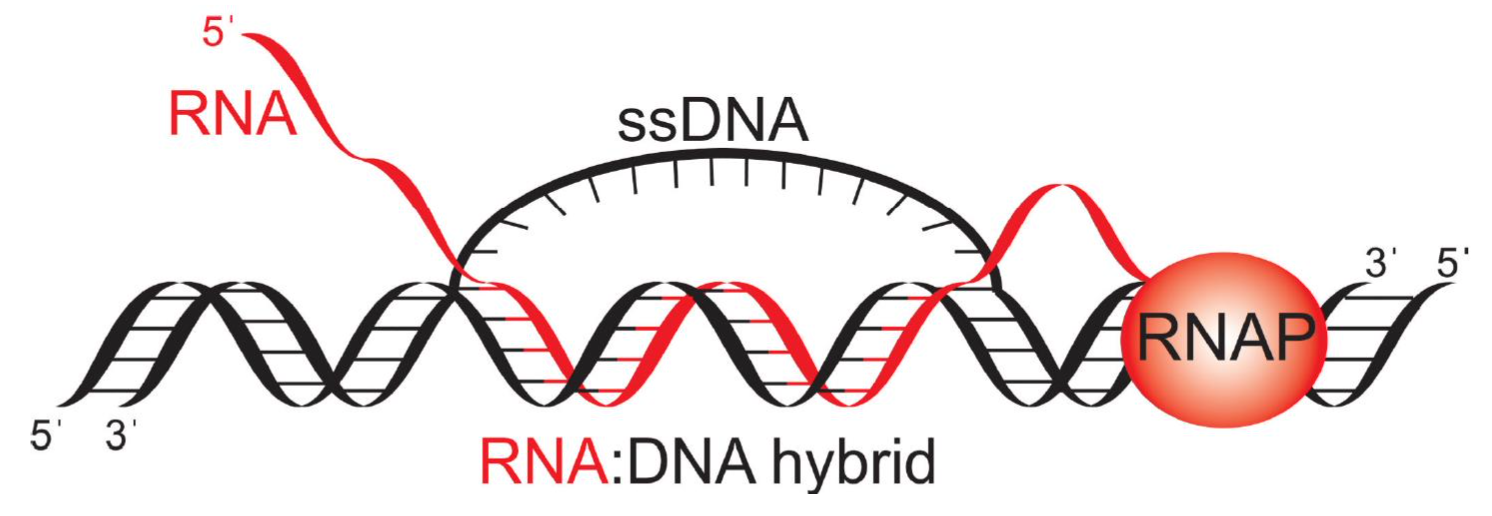
\includegraphics[width=0.5\textwidth]{../_resources/Screen_Shot_2022-11-23_at_09-53-33.png}
\caption{Hamperl and Cimprich, DNA Repair, 2014}
\label{fig:hybrid}
\end{figure}

High G density in the non-template DNA strand promotes R-loops formation. RNA:DNA hybrids rich in RNA-G/DNA-C ratio are more stable than DNA:DNA duplex of the same sequence.

Transcription unwinding results in topological stress and generation of DNA supercoils.
\begin{itemize}
\tightlist
\item
  Positive toroidal supercoils: dsDNA is tightly packed
\item
  Negative toroidal supercoils: loose DNA, predisposition to RNA insertion.
\end{itemize}

Superhelical stress can favor, and be mitigated by, R-loops formation.

In highly transcribed genes we witness histone turnover, which is favored by negative supercoiling. R-loops formation inhibits nucleosomes redeposition weakening surrounding nucleosome-DNA contacts.

G-rich sequences and negative supercoiling can promote the formation of R-loops. In addition, to win competition with the non-template strand, the stability of the sequence is important $\rightarrow$ G-quadruplexes highly increase stability.

\textbf{G-quadruplexes:} 4 guanines interacting by hydrogen bonds (Hoogsteen) on the same plane (planar quartet). We can find parallel G4 or antiparallel G4 (based on the orientation of guanines).

R-loops are typically formed co-transcriptionally (cis) but formation in trans has been reported and expected e.g.~Cas9 pathway or ncRNA with unwinding promotion.

\hypertarget{r-loop-degradation}{%
\subsection{R-loop degradation}\label{r-loop-degradation}}

TREX complex: mediates transcript export for splicing and translation. If we remove THO subunit, we impair trex and formation of R-loops $\rightarrow$ limiting the amount of naked RNA in the cells prevents R-loops accumulation.

R-loops are also actively eliminated by specific enzymes:
\begin{itemize}
\tightlist
\item
  RNAse H1/2 recognize and degrade R-loops
\item
  RNA:DNA helicases e.g.~Sen1/SETX
\end{itemize}

\hypertarget{r-loop-recognition-and-distribution}{%
\subsection{R-loop recognition and distribution}\label{r-loop-recognition-and-distribution}}

\textbf{DRIP-seq:} The monoclonal S9.6 antibody revealed thousands of R-loop hotspots in human genome. R-loops can be found in:
\begin{itemize}
\tightlist
\item
  highly transcribed genes (as rate of transcription can influence loop formation for negative torsional stress)
\item
  telomeres: G-rich non-template strand, C-rich template strand
\item
  ORF: proposed function at termination sites for termination factor recruitment e.g.~chromatin remodeling.
\end{itemize}

! Pull down is performed after sonication, mechanic stress on DNA $\rightarrow$ bias. A good part of the signal could be coming from dsDNA. Over the years, improvements to the method were done e.g.~bisulphide for T$\rightarrow$U, only finds RNA.

Endogenous R-loop structures are also detected by \textbf{R-ChIP}: a catalytically dead RNASEH enzyme can be expressed in cells, able to recognize but not degrade. We visualize R-loops endogenously. Bias: RNASE can be recruited on paused sites, the technique can only applied in cell lines.

R-ChIP and DRIP-seq experiments reveal R-loops enrichment at promoter regions and TSS. Approximately 60\% human promoters are associated with a CGI - CGI methylation, which generally associates with gene silencing.

R-loops form in human CpG island promoters with G-rich sequence at the non-template strand (GC skew) regulate DNA methylation.

\hypertarget{vim-antisense1}{%
\subsection{VIM-antisense1}\label{vim-antisense1}}

VIM is an intermediate filament in mesenchymal cells (EMT process). There is a presence of a CpG island. Usually with antisense the transcription of the sense collides due to sterical hindrance (overlapping). In this case, the antisense is polyadenylated and nuclear, while the sense is cytoplasmic. The expression of the antisense is associated with down-regulation of the sense gene. Depletion of VIM-AS1 causes downregulation of the VIM gene expression provoked by methylation (Figure \ref{fig:vim}).

\begin{figure}
\centering
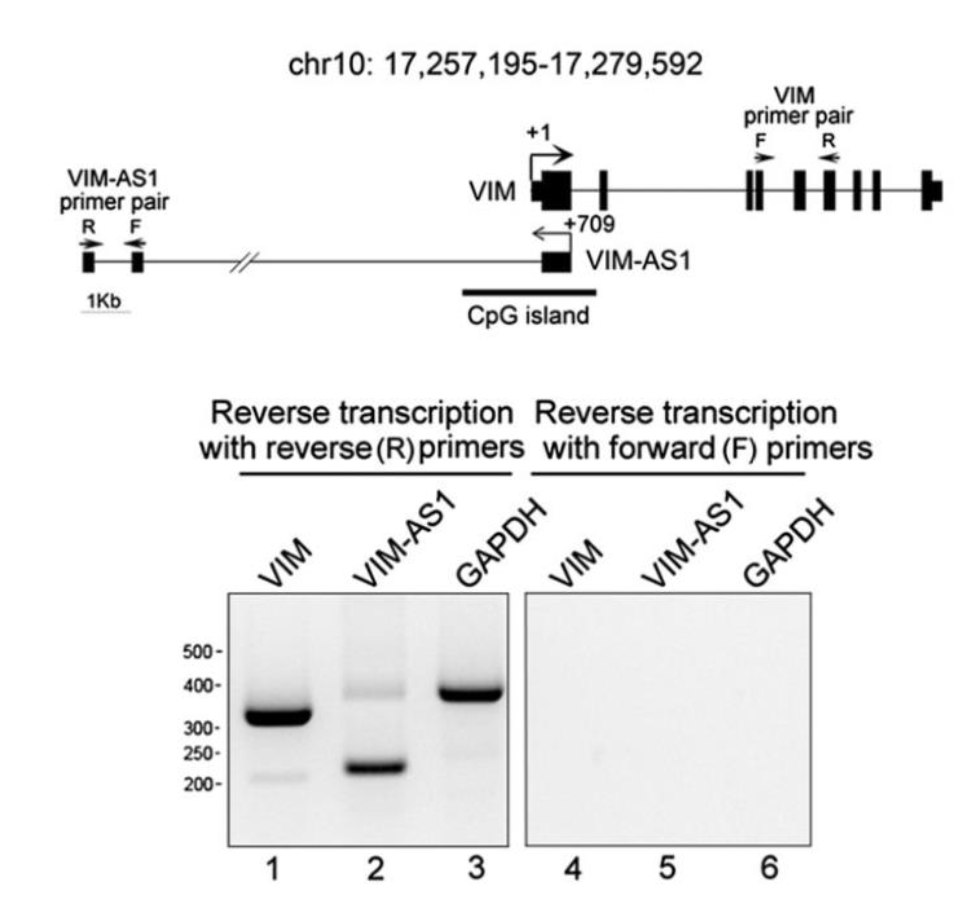
\includegraphics[width=0.5\textwidth]{../_resources/Screen_Shot_2022-11-23_at_10-18-00.png}
\caption{}
\label{fig:vim}
\end{figure}

The two transcripts can be visualized through FISH with different fluorophores. By combining this technique with the inhibition of transcription VIM disappears, while VIM-AS1 is more stable. This could be due to the fact that it is engaged with a R-loop structure. The genomic region between the two TSSs shows GC skew sequences.

R-loop formation is dependent on the antisense transcript. RNaseH1 overexpression inhibits VIM and VIM-AS1 expression. R-loop structures promote VIM expression by impairing nucleosome occupancy and favoring the binding of transcription factors.

Expression of antisense and R-loop associate with open chromatin. By blocking R-loops or inhibiting VIM-AS1 at FNkB TF binding sites accessibility is reduced and the recruitment of the TF at the locus is impaired.

\textbf{Main findings:}
\begin{itemize}
\tightlist
\item
  loop formation by antisense RNAs at CpG island containing promoters can impair DNA methylation at these promoter sequences
\item
  decrease nucleosome occupancy and favor binding of the transcription factor NF-kB to the promoter of Vimentin gene promoting transcription of the sense gene
\end{itemize}

R-loops can regulate gene expression by multiple mechanisms: repressing chromatin modifiers, activating chromatin modifiers and chromatin regulating complexes. They arise naturally and have multiple physiological effects e.g.~DNA repair, replication and gene expression, and are therefore tightly regulated. R-loops are generally transient and regulated by enzymatic activity; under certain conditions, R-loops become de-regulated and accumulate in cells.

\hypertarget{hottip-dependent-r-loop-formation-regulates-ctcf-boundary-activity-and-tad-integrity-in-leukemia}{%
\subsection{HOTTIP-dependent R-loop formation regulates CTCF boundary activity and TAD integrity in leukemia}\label{hottip-dependent-r-loop-formation-regulates-ctcf-boundary-activity-and-tad-integrity-in-leukemia}}

In vertebrates the Hox genes are located contiguously in clusters. Hox genes are expressed in a tightly regulated spatio-temporal manner during embriogenesis. They posses the homeobox domain and are divided into 4 clusters. The spatio-temporal expression is also observed in human primary fibroblast from different sites. 5C chromosome interaction highlights the presence of the \emph{posterior domain}. Differentiated cells (distal cells from limbs) have a distinct pattern with respect to proximal cells (from lung): in distal Pol II signal and H3K4me is observed in the first HOTTIP region, while the opposite patterns is present in proximal cells (HOTAIRM1 region at 3' $\rightarrow$ lncRNA interacting with chromatin remodelling complex).

HOTTIP stands for HOXA transcript at the distal tip. HOTTIP lncRNA stimulates the transcription of HoxA genes by enforcing H3K4me3 chromatin modification (Figure \ref{fig:hottip}).

\begin{figure}
\centering
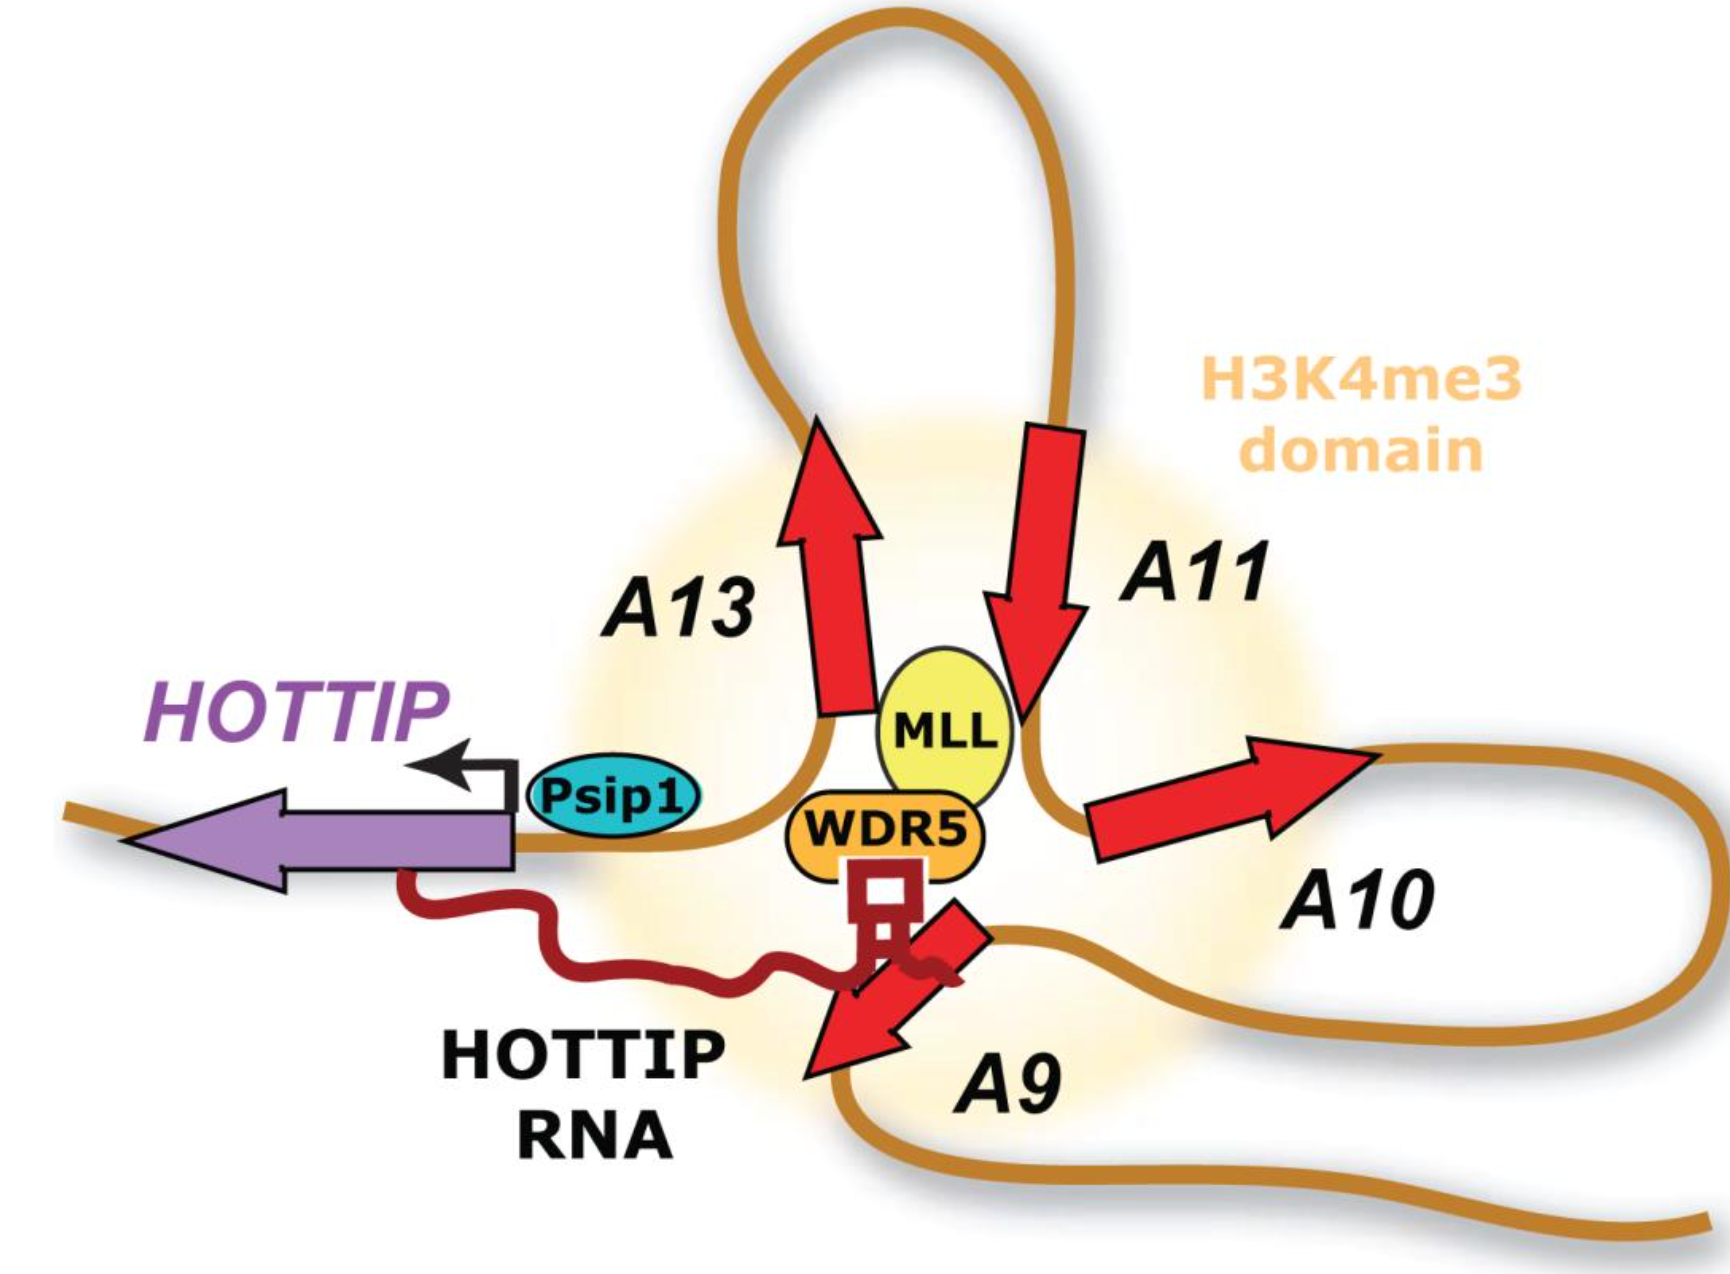
\includegraphics[width=0.5\textwidth]{../_resources/Screen_Shot_2022-11-25_at_11-49-03.png}
\caption{}
\label{fig:hottip}
\end{figure}

Chromosomal looping brings HOTTIP RNA in close proximity to the HOXA genes. HOTTIP lincRNA binds to and targets WDR5--MLL complexes to the HOXA locus, leading to transcription activation. The mutual interdependence between HOTTIP RNA and WDR5-MLL creates a positive feedback loop that maintains the ON state of the locus.

HOX genes are mutated or deregulated in different cancers and play active roles in tumorigenesis. HOXA genes are expressed in hematopoietic stem cells and progenitor cells while downregulated during differentiation. Abnormal HOXA gene activation is a common feature of acute myeloid leukemia (AML). HOXA9 and HOXA10 genes are frequently aberrantly activated in AML patients. Dysregulation of HOXA genes (e.g., HOXA9) is a driving mechanism for hematopoietic deregulation and leukemogenesis. Overexpression of HOXA9 is a poor prognostic marker in leukemia patients while its downregulation is a favorable predictor of AML patient outcome. The mechanisms regulating HOXA genes expression in AML patients is under investigation.

A transition from repressive to active chromatin is detected within the HOXA locus in AML patients. Among A7 and A9 we observe a sort of boundary, mainly regulated by insulator sequences $\rightarrow$ the CTCF binding site located between HOXA7 and HOXA9 genes may regulate the aberrant activation of the HOXA9-13 genes in AML cells.

Deletion of the CTCF binding site between HOXA7/9 genes (CBS7/9+/-) alters HOXA gene expression in AML cell lines. The homozygous deletion was incompatible with cell survival, so heterozygous was used. ChIP-seq analyses of CBS7/9+/- cells show altered chromatin structure in the HOXA9-13 domain but not in the HOXA1-7 locus, consistent with a loss of boundary function. 4C-seq data indicate decreased HOXA9 interaction with proximal genomic sites.

\textbf{CBS7/9+/- is important to regulate the chromatin structure and the expression of HOXA9-13 genes in AML cells.}

Dysregulation of CBS7/9 boundary inhibits leukemic cell proliferation and prolongs survival time of transplanted NSG mice. In addition to the local effect on chromatin marks and structure, a significant number of dysregulated genes was observed e.g.~oncogenic pathways RUNX1, SOX involved in myeloid activation.

Attenuation of the chromatin boundary disrupts the active chromatin domain and perturbs oncogenic gene expression in AML, in part by disrupting the HOXA9 oncogenic pathway. The CBS7/9 boundary located at the edge of the TAD encompassing the posterior HOXA genes establishes and maintains aberrant chromatin signatures and expression of the posterior HOXA genes to facilitate myeloid leukemogenesis. The elimination of CTCF fosters the formation of aberrant protein.

\emph{Can a normal CTCF boundary be hijacked to control oncogenic chromatin domain and transcription profiles for leukemic transformation and progression?}

HOTTIP--/-- perturbs HOXA gene-mediated oncogenic transcription program, we observe oncogene downregulation. The KO is able to recapitulate the effect of CBS7/9 on HOXA. In wt AML cells we can identify the anterior and posterior domain, in KO cells we observe a change in the posterior domain.

HOTTIP lncRNA is aberrantly expressed in a subset of AML patients and cells. NPM1-mutated (NPM1C+)or MLL-rearranged (MLLr+) AML cases (n = 76) exhibited elevated levels of HOTTIP expression. Survival rate was inversely correlated with HOTTIP expression.

Activation of HOTTIP rescues the HOXA gene chromatin defects in the CBS7/9+/-- AML cells.

HOTTIP transgenic expression in hematopoiesis leads to AML-like disease and promotes hematopoietic transcription programs.

\textbf{Conclusions}
\begin{itemize}
\tightlist
\item
  HOTTIP expression alters HOXA genes containing TADs and HOXA genes expression
\item
  HOTTIP KO affects leukemic transcription program while HOTTIP overexpression leads to AML-like disease
\item
  HOTTIP is aberrantly expressed in AML patients
\end{itemize}

\hypertarget{hottip-lncrna-promotes-hematopoietic-stem-cells-self-renewal-leading-to-aml-like-disease-in-mice}{%
\subsection{HOTTIP lncRNA Promotes Hematopoietic Stem Cells Self-Renewal Leading to AML-like Disease in Mice}\label{hottip-lncrna-promotes-hematopoietic-stem-cells-self-renewal-leading-to-aml-like-disease-in-mice}}

CHIRP: reminds us of ChIP for crosslinking and sonication. Instead of using antibodies, they use specific probes for the RNA of interest with tilling oligos (bp with different regions of the RNA, increased yield of the pull down). At the end of the protocol we obtain RNA.

HOTTIP interactome isolated from AML cells contains CTCF/cohesin complex and R-loop- associated proteins.

HOTTIP KO resulted in a significant reduction of R loops and HOTTIP binding sites, especially when cobound to CTCF.

No signal from GRO-Seq $\rightarrow$ HOTTIP KO disrupted CTCF and cohesin TAD boundaries containing AML oncogenes such as $\beta$-catenin (CTNNB1). At these boundary sites HOTTIP RNAs form R-loops in trans. HOTTIP-mediated R-loop formation directly contributes to CTCF boundary activity.

R-loops disruption at the CBS-u2 boundary site impairs proliferation of AML cells.

\hypertarget{dna-damage}{%
\section{DNA damage}\label{dna-damage}}

Single stranded DNAs are more susceptible to chemical modifications, strand breaks, mutagen sensitivity and secondary structure than dsDNAs. Also dsDNA is undergoing spontaneous chemical modifications. Basically, any covalent bond in DNA molecule can be attacked by a water molecule. It has been estimated that there are thousands of spontaneous lesions in our cells e.g.~depurination (G$\rightarrow$sugar phosphate) or deamination (C$\rightarrow$U). Spurious methylation can occur in bases different from cytosine; when a RNA pol II passes through modified bases, we can observe a stall or the insertion of an erroneous base, leading to mutations. The addition of chemical groups occurs when bases react with oxygen species e.g.~guanine + adduct radical gives 8-hydroxyguanine.

\textbf{Base excision repair} (BER) pathway eliminates modified bases or depurinated nucleotides (Figure \ref{fig:ber}).

\begin{figure}
\centering
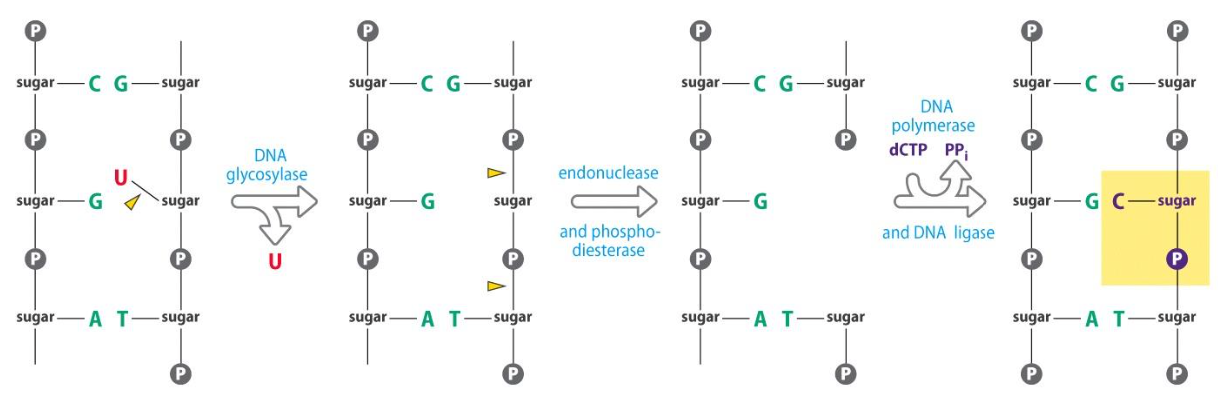
\includegraphics[width=0.5\textwidth]{../_resources/Screen_Shot_2022-11-30_at_08-49-05.png}
\caption{Base excision repair}
\label{fig:ber}
\end{figure}

The chemical modification rate in oligonucleotides depends on cation concentration, pH, and other experimental conditions. Roughly 5\% of the genome can be occupied by R-loops.

\hypertarget{r-loop-modified-bases}{%
\section{R loop modified bases}\label{r-loop-modified-bases}}

Modified bases within R-loops that are not properly repaired form nicks and breaks (this step requires dsDNA) $\rightarrow$ replication and transcription stops. R-loops accumulation associates with genome instability due to the spontaneous base modifications occurring at ssDNA and the ensuing processing events leading to nicks and breaks.

\begin{figure}
\centering
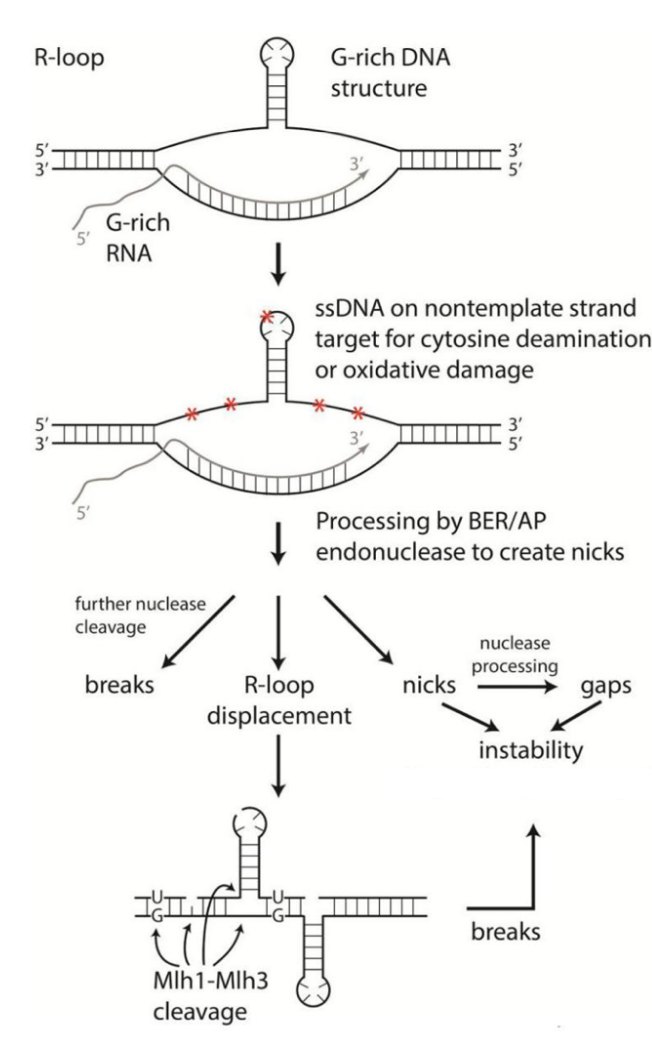
\includegraphics[width=0.3\textwidth]{../_resources/Screen_Shot_2022-11-30_at_08-51-07.png}
\caption{R loop repair}
\label{fig:rrep}
\end{figure}

Thanks to R-loop displacement, BER can excite modified bases; this provokes a misaligned dsDNA, leading to breakages - especially if loops are hit by modifications - and genome instability (Figure \ref{fig:rrep}).

R-loops can lead to nicks and breaks (DSBs) also due to the activity of the AID/APOBEC cytidine deaminases (catalyzed modifications). \textbf{Activation-induced cytidine deaminase} (AID) promotes somatic hypermutation and class switch recombination of immunoglobulin (Ig) genes in germinal center (GC) B cells. AID off-target activity has been implicated in malignant transformation of GC-derived B cell lymphomas.

C$\rightarrow$U is meant to be, as cells want to induce mutation in a random manner to achieve hypervariability. In particular, several cancers are characterized by APOBEC signatures, which are a key source of mutation e.g.~chromosome instability in early breast and lung cancer evolution. Not only \emph{spontaneous} base modifications but also cytosine deamination catalyzed by \textbf{APOBECs} can lead to nicks and breaks within R-loops structures leading to genome instability.

\hypertarget{apical-kinases}{%
\subsection{Apical kinases}\label{apical-kinases}}

Cells have evolved the \textbf{DNA damage response} (DDR) in order to combat threats
posed by DNA damage. Breaks are sensed by apical kinases: \textbf{ATM}, \textbf{ATR} and \textbf{DNA-PKcs} (Figure \ref{fig:apical}). Phosphorylated serine or threonine residues followed by glutamine (S/T-Q) S/T-Q sites are present in ATM, ATR and DNA-PKcs for autophosphorylation. They all contain a kinase domain at the C-terminal. Cancer cells and immunodeficient cells (mutated in these genes) are more susceptible to radiation, since the recognition of ds breaks is impaired $\rightarrow$ radiotherapy would result in important side effects.

ATM, ATR and DNA-PKcs require specific co-factors for their recruitment to
damaged DNA. ATM is linked to a trimeric complex (MRN), where MRE11 is the endo/exo nuclease, RAD50 recognizes dsDNA and NBS1 is full of PPinteracting domain (ATM recruitment). ATR is recruited to dsbreaks when they are processed, so ssDNA bound by RPA (aspecific marker), bound by ATRIP co-factor.

\begin{figure}
\centering
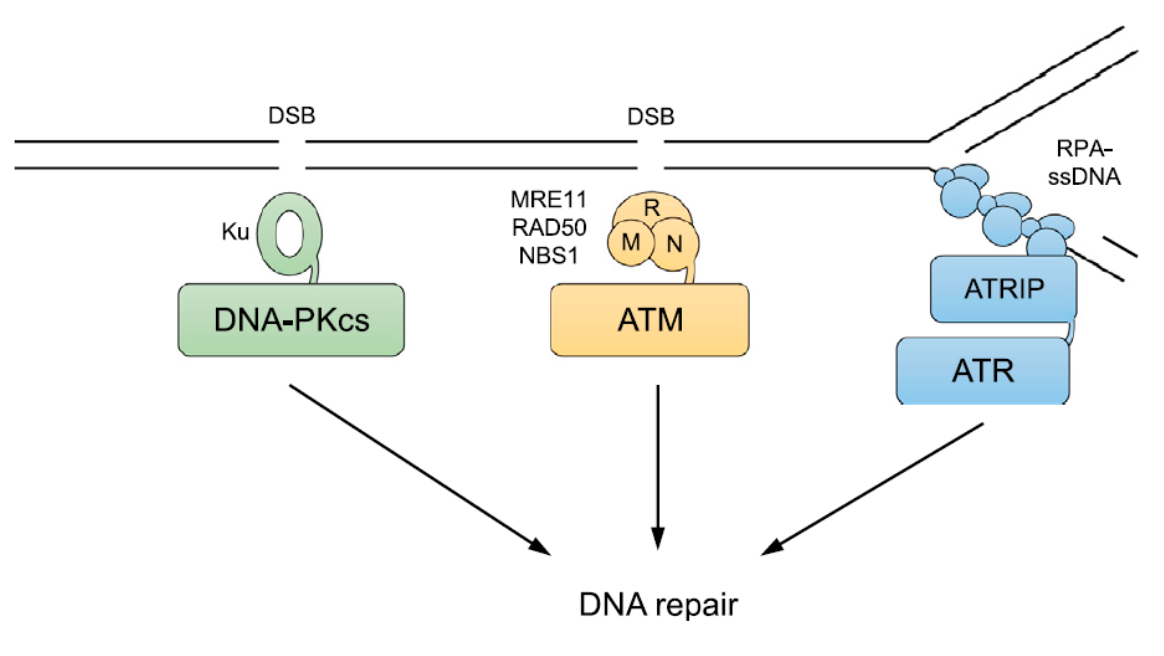
\includegraphics[width=0.5\textwidth]{../_resources/Screen_Shot_2022-11-30_at_09-11-05.png}
\caption{Apical kinases}
\label{fig:apical}
\end{figure}

They are also involved in cell cycle control, DNA replication, transcriptional regulation and RNA metabolism. It orchestrates real cell response.

\textbf{DNA-PKcs} promotes NHEJ of DSBs: DNA-PKcs phosphorylation allows the recruitment of downstream NHEJ core factors, leading to DNA-end ligation by LIG4. This pathway is fast and can be used in all cell cycle phases.

ATM activation promotes a signaling cascade on damaged chromatin. MRN recruits ATM, which can phosphorylate hundreds of different targets, which are themselves kinases $\rightarrow$ kinase cascade. The first event is the phosphorylation of H2AX, leading to $\gamma$ H2AX marker for DNA damage. MDC1 is recruited and phosphorylation, additional MRN recruitment and feed-forward mechanism. Gamma H2AX can spread megabases, self sustaining cycle enhancing the reaction to ds break. TIP60 activates ATM through acetylation.

53BP1 is an effector of DNA damage response (reaction of the cell to ds break, enabling sensing) and DNA repair mechanism (fix the break) $\rightarrow$ NHEJ activation. Among the ATM targets we have BRCA1 (scaffold molecule and ubiquitinligase) and CtIP (endonuclease), which are phosphorylated $\rightarrow$ signal for the cell to activate homologous recombination (requires the sister chromatid, S phase only).

\begin{figure}
\centering
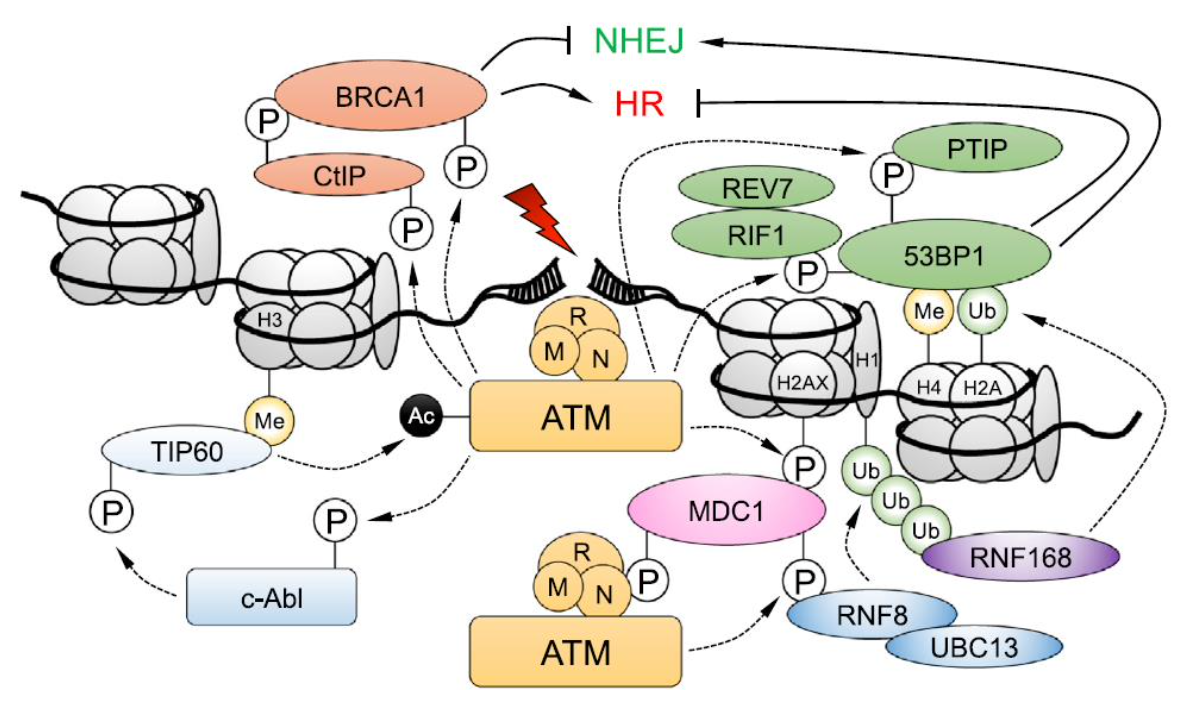
\includegraphics[width=0.6\textwidth]{../_resources/Screen_Shot_2022-11-30_at_09-16-55.png}
\caption{Blackford and Jackson, \emph{Mol Cell}, 2017}
\end{figure}

\textbf{BRCA1 and 53BP1 determine the choice of repair mechanism between NHEJ
and HR.} The decision between NHEJ and HR is also determined by several factors including cell cycle phase, chromatin state, genetics. NHEJ is ``error prone'' (but not in the classic pathway, alternative one), while homologous recombination is error free.

\begin{figure}
\centering
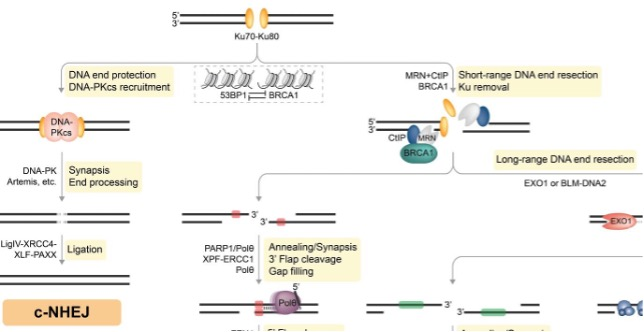
\includegraphics[width=0.7\textwidth]{../_resources/Picture1.jpg}
\caption{Trenner and Satori, Frontiers in Oncology 2019}
\end{figure}

DNA damage response integrates regulation of the cell cycle, which is blocked in order to prevent mitosis. It is necessary to allow repair mechanism to act before resuming the cell cycle. Cell cycle is regulated by CHK2 (kinase phosphorylating CDK29) and p53.

The key signal for the cell in the context of repair comes from DNA ends; telomere mask chromosome ends from being recognized as double-strand breaks.

DNA damage response (DDR) involves DNA lesion recognition followed by a signaling cascade to promote DNA repair. The effectors lead to transient checkpoint, cellular senescence and apoptosis.

The roles of\textbf{ PARP1} (poly(ADP-ribose) polymerase 1) in detection and repair of DNA double-strand breaks are several. It is recruited to ds break and adds poly(ADP-ribose) chains. The recruitment of covalently and non-covalently modified proteins to site of DNA damage allows for repair of ssDNA nicks and breaks, sd breaks and chromatin modifications. PARP is also associated with ATM itself and is involved in HR, cNHEJ and aNHEJ. Although it is not the only activating mechanism of BRCA, it supports it to the break and lead to strand invasion and resolution.

Summarizing, defects in DSB repair e.g.~loss or Xrcc4, LIG4, BRCA1 lead to chromosome instability and accumulation of mutation $\rightarrow$ defective checkpoints, cancer.

\hypertarget{topoisomerases}{%
\subsection{Topoisomerases}\label{topoisomerases}}

Programmed ssDNA and dsDNA breaks occur during transcription. As we have mentioned, positive and negative torsional stress generate forces opposing the direction of pol II. \textbf{Topoisomerase cleavage complexes} (TOPcc) assemble at sites of topological stress. They are tightly regulated to minimize deleterious cleavage complexes - their activity is impeded by nucleosomes. They are recruited to chromatin via interaction with chromatin remodelling complexes (SWI/SNF), histone chaperones (FACT) and helicase enzymes (WRN).

TOP1 triggers SSBs or nicks, TOP2 induces DSBs. Both perform breakage in a controlled manner and once torsion is released they can exert ligation activity. During transcription TOP1 and TOP2 enzymes relieve positive supercoils, while TOP1 and TOP3 counteract negative supercoils.

\hypertarget{a-topoisomerase-iib-mediated-dsdna-break-required-for-regulated-transcription}{%
\subsubsection{A topoisomerase IIb-mediated dsDNA break required for Regulated Transcription}\label{a-topoisomerase-iib-mediated-dsdna-break-required-for-regulated-transcription}}

Biotin-dUTP labelying by terminal deoxy $\rightarrow$ only if a break is present. Amplification of the promoter region and not of the ORF, signaling the presence of a break in the promoter leading to the recruitment of PARP. However the break is transient, after 10 minutes it disappears (Figure \ref{fig:biot}).

\begin{figure}
\centering
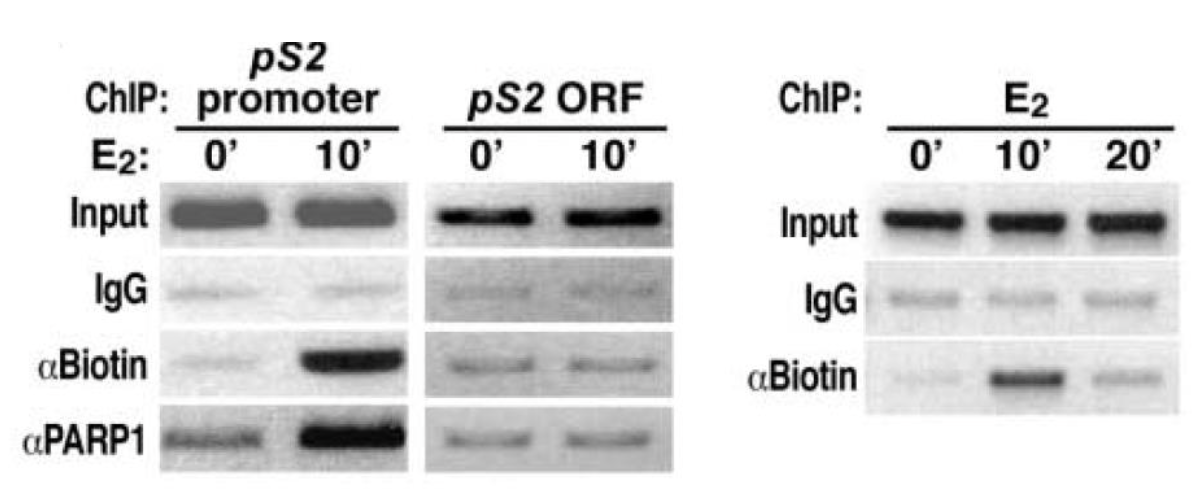
\includegraphics[width=0.5\textwidth]{../_resources/Screen_Shot_2022-11-30_at_10-03-17.png}
\caption{Screen Shot 2022-11-30 at 10-03-17.png}
\label{fig:biot}
\end{figure}

DSBs are induced transiently on the pS2 promoter upon estrogen treatment. Transcriptional activation associates with transient and local formation of DNA double strand breaks. TopoII$\beta$-mediated DSBs at the pS2 promoter is required for pS2 transcription. If we block topoisomerases, machinery for transcription is not recruited. The presence of DNAPK persists for a while after the resolution of the break, this does only mean that the signal is spreading.

TopoIIb/PARP-1 complex in nuclear receptor-mediated gene regulation TopoII mediated DSB and in PARP-1 activity serves as mechanism for gene transcription upon ligand or signal- dependent stimulation. PARP1 activity promotes removal of histone H1 from the ERE-containing nucleosome supporting transcription initiation.

\hypertarget{brca1}{%
\subsubsection{BRCA1}\label{brca1}}

Sometimes, pathological topoisomerase 2 sites are observed. TOP2 is required for ER-medited transcription. Occasional estrogen-induced pathological TOP2 occur with DSBs covalently associated with the enzyme. BRCA1 participates in resolving these structures promoting genome integrity. In the absence of BRCA1, estrogen exerts a genotoxic effect with accumulation of DSBs during cell divisions.

The roles of BRCA1 in the maintenance of genome integrity and regulation of transcription may be the key of its tissue specific tumor suppressor function.BRCA1 has an ubiquitinylase domain (RING) and a huge number of interacting proteins. BRCA1 drives a transcriptional program supporting differentiation of luminal progenitors to mature luminal cells. BRCA1 interaction inhibits ER$\alpha$ activity directly and by promoting mono-ubiquitination of ER$\alpha$. BRCA1 mutant progenitors are aberrantly proliferative and defective in differentiation giving rise to tumors of luminal origin. Cells with LOH in BRCA1 usually show basal-like tumor activity.

\hypertarget{stark-et-al.}{%
\subsubsection{Stark et al.}\label{stark-et-al.}}

24h estrogen treatment activates DNA damage response pathways and associates with DSBs in MCF7 cells. \textbf{Comet assay:} cells are lysate, nuclei as inserted in an agarose pad and placed under an electrophoretic chamber (no fragmentation): if there are ds breaks it will move a little bit, we will observe a ``comet'' signal. In 24 hours cells can cycle and perhaps this is not the same break as topoisomerase II. Long term estrogen treatment results in greater DDR activation than short term treatments.

DNA damage induced by long term estrogen treatment is replication dependent, the more the cell proliferate, the more the DNA damage response is activated. If we add a Cdc7 inhibitor, DNA damage response activation is impacted. Flavopiridol (inhibits Cdk9) results in Pol II elongation impairment, but does not affect replication.

Estrogen induces R-loops formation at ER responsive genes. The induction of R loop was depending on ER target genes. Gene responsive to estrogen are enriched in genomic rearrangements in breast tumors. 

Estrogen induced R-loops colocalize with DNA damage markers on chromatin. Proximity ligation assays suggest that estrogen induced R-loops occur on chromatin marked by DNA damage.

RNaseH expression reduces estrogen induced DNA damage. RNaseH expression reduces estrogen induced DSBs. R-loops may be involved in DNA damage induction DSBs formation in breast cancer cells upon estrogen treatment.

\textbf{Summary}
\begin{itemize}
\tightlist
\item
  Estrogen treatment induces replication and transcription dependent DNA damage
\item
  DNA damage and DSBs induced by estrogen stimulation are linked to R-loop formation at ER responsive genes
\item
  Breast cancer rearrangements are enriched at estrogen responsive loci where R-loops are detected upon estrogen treatment
\item
  Many DSBs that accumulate upon estrogen treatment are R-loops dependent
\item
  Estrogen stimulation leads to genome instability through R-loops formation and in a DNA
  replication dependent manner
\item
  Also highlights an «alternative» mechanism by which a transcriptional program plays a role in genome stability in cancer
\end{itemize}

\hypertarget{dna-damage-signaling-activation-during-tumorigenesis}{%
\section{DNA damage signaling activation during
tumorigenesis}\label{dna-damage-signaling-activation-during-tumorigenesis}}

If we think about it, one of the hallmarks of cancer is gene instability (chromosome re-arrangement), which need some sort of break for it to happen. Compare DNA in pre-cancerous and cancerous tissue (and normal).
The more aggressive is the cancer, the lest the response of DNA repair genes. 

\begin{figure}
\centering
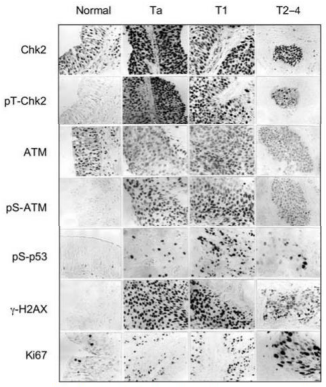
\includegraphics[width=0.4\textwidth]{../_resources/b6767c28ca4d9960f33b0d725382b694.png}
\caption{Difference in response of DNA repair genes based on the aggressiveness of the cancer.}
\label{fig:repair}
\end{figure}

Increased recruitment of DNA repair increases gene instability. pT-Chk2 detection: absent (white), detected at low (light grey), medium (dark grey) or high (black) levels (figure \ref{fig:pT-Chk2}):

\begin{figure}
\centering
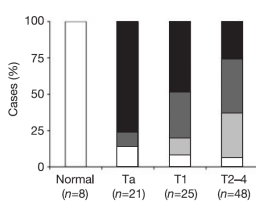
\includegraphics[width=0.35\textwidth]{../_resources/168deb888ea330cd5cfa4cd813e7260d.png}
\caption{Levels of pT-Chk2}
\label{fig:pT-Chk2}
\end{figure}

However, the DDR in pathways are impaired (Figure \ref{fig:DDR}).

\begin{figure}
\centering
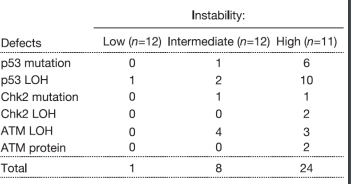
\includegraphics[width=0.5\textwidth]{../_resources/eca41a16e9bce1f13534cbefd1902bbe.png}
\caption{DDR in pathways are impaired}
\label{fig:DDR}
\end{figure}


\hypertarget{which-tumorigenic-events-trigger-activation-ddr-very-early-in-tumorigenesis}{%
\subsection{Which tumorigenic events trigger activation DDR?}\label{which-tumorigenic-events-trigger-activation-ddr-very-early-in-tumorigenesis}}

There are different ways to induce oncogenes, what we know is that upon activation cell proliferate until they reach a plateau (oncogene
induced senescence: persistent activation of DDR pathways.) 
Different form of replicative senescence (telomers). There is no way to recover from it (both oncogenic or replicative), unless we act \emph{genetically} (figure \ref{fig:activation}).

\begin{figure}[h!]
\centering
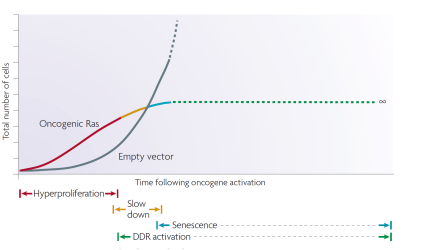
\includegraphics[width=0.5\textwidth]{../_resources/e5bec01cb6c2d9a42b67721810b931fb.png}
\caption{Oncogenes}
\label{fig:activation}
\end{figure}

Main features of senescent cells: 
\begin{itemize}
\tightlist
\item Permanent growth arrest 
\item Persistent DNA damage response signaling (DDR) 
\item Increase in size (even of two
fold)
\item Expression of $\beta$-galactosidase ($\beta$-gal) 
\item Formation of
senescence-associated heterochromatin foci (SAHF) 
\item Secretion of growth factors, proteases, cytokines (senescence-associated secretory phenotype: SASP, underlying the fact that they can promote inflammation. Cytokines are pro-proliferative messages.)
\end{itemize}

\hypertarget{oncogene-induced-senescence-cells}{%
\subsection{Oncogene induced senescence
cells}\label{oncogene-induced-senescence-cells}}

\begin{figure}[h!]
\centering
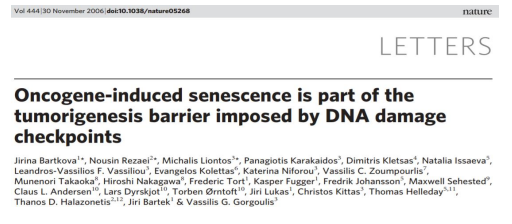
\includegraphics[width=0.6\textwidth]{../_resources/76f900cd20da07b3fcbf3ae29e21596b.png} 
\label{fig:senescence1}
\end{figure}
%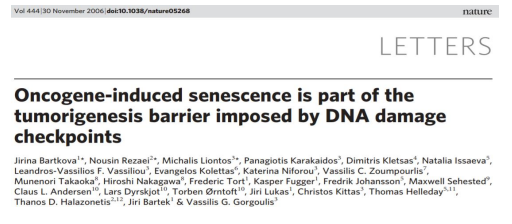
\includegraphics{../_resources/76f900cd20da07b3fcbf3ae29e21596b.png} 

DDR induced by oncogene expression acts as a barrier to cell proliferation.
We can bypass this barrier by over expressing genes like RAS, or
downregulating genes like p53:

\begin{figure}[h!]
\centering
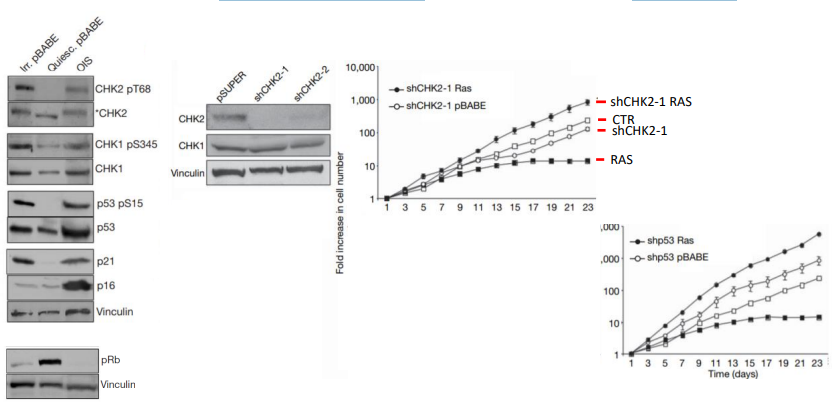
\includegraphics[width=0.5\textwidth]{../_resources/b0a12e30eb68712a5f227c5bff2c9424.png} 
\label{fig:senescence2}
\end{figure}
%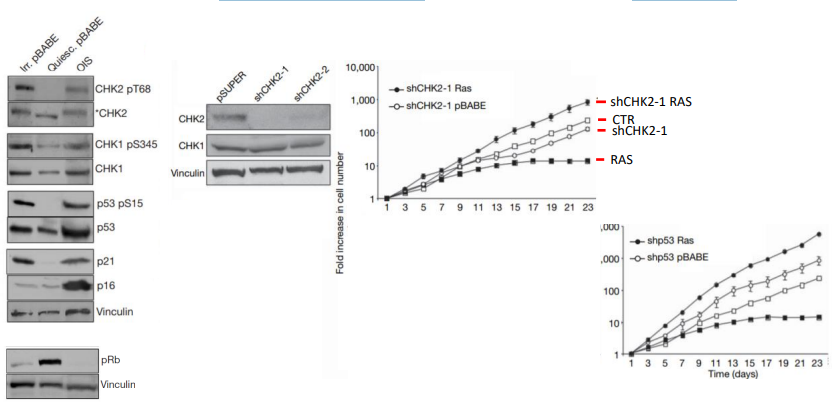
\includegraphics{../_resources/b0a12e30eb68712a5f227c5bff2c9424.png}

But what is triggering DDR upon oncogene expression?

Experiment: two cell lines (one with RAS). Black bars: transduction
efficiency; grey bars: BrdU; red bars: pS/TQ.

\begin{figure}[h!]
\centering
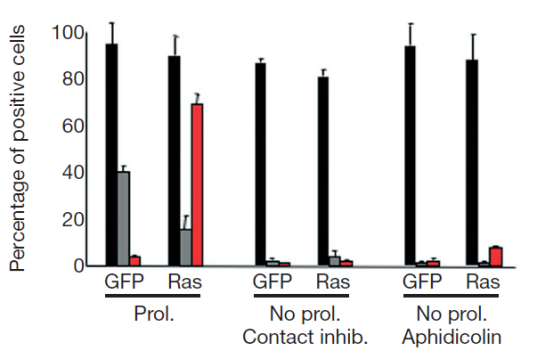
\includegraphics[width=0.5\textwidth]{../_resources/f78ec4683d1e9e77bb74c4f6a372ac8b.png}  
\label{fig:senescence}
\end{figure}
%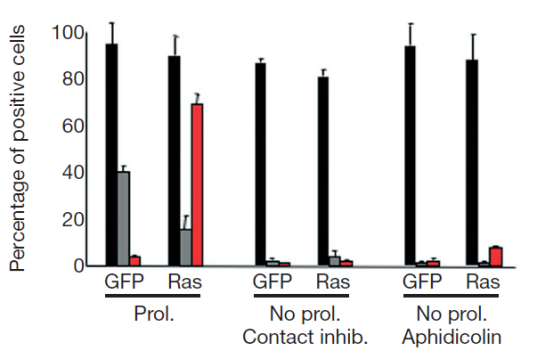
\includegraphics{../_resources/f78ec4683d1e9e77bb74c4f6a372ac8b.png} 

In pBABE: normal signals, one for each probe. In treated fibroblasts, we
see something strange. Many sites of transcription, even if the
centromeres are stile two (no anaeuploidy).

\begin{figure}[h!]
\centering
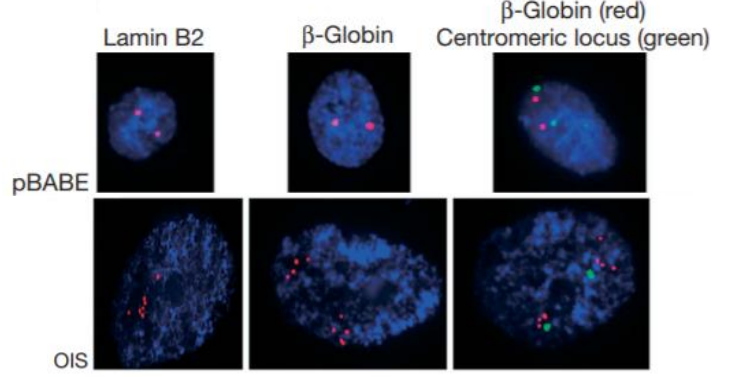
\includegraphics[width=0.5\textwidth]{../_resources/b399b9d2beb17cee2a4d602739e97b08.png} 
\label{fig:senescence}
\end{figure}
%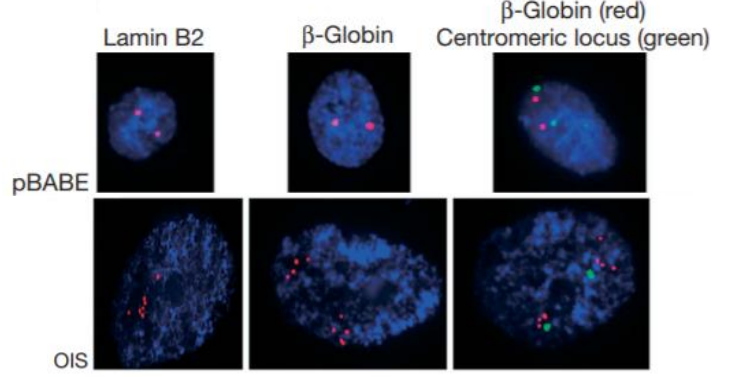
\includegraphics{../_resources/b399b9d2beb17cee2a4d602739e97b08.png}

The link between activation of oncogenes and senescence has something to
do with DNA replication stress. In precancerous lesions that typically
retain wild-type p53 function, the oncogene induced DNA damage elicits
p53- dependent apoptosis and/or senescence, which limits growth of the
lesion. When the function of p53 is lost, cells can escape its apoptotic
and/or senescence effects, and the precancerous lesion can become
cancerous.

\begin{figure}[h!]
\centering
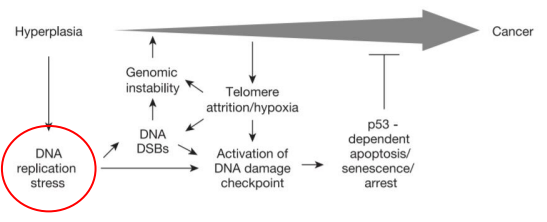
\includegraphics[width=0.5\textwidth]{../_resources/504253851a3ef8203e6353a576814cc4.png} 
\label{fig:senescence}
\end{figure}
%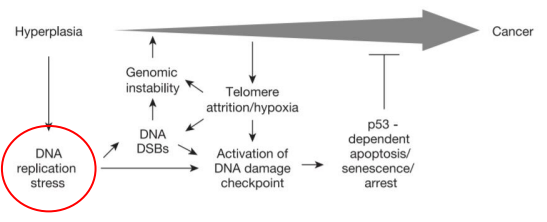
\includegraphics{../_resources/504253851a3ef8203e6353a576814cc4.png}

\hypertarget{replication-stress}{%
\subsubsection{Replication stress}\label{replication-stress}}

How does replication start? It is tightly regulated in time and space.
Two main steps: licensing and origin finding. The input for initiation
is phosphorilation, mediated by a bunch of kinases (like CDK) (figure \ref{fig:rep}).

\begin{figure}[H]
\centering
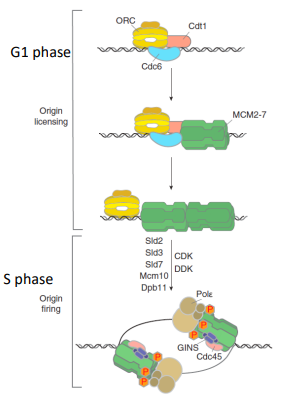
\includegraphics[width=0.4\textwidth]{../_resources/cf33180a017e8d51c049566410ac8b20.png}
\caption{Normal replication start}
\label{fig:rep}
\end{figure}
%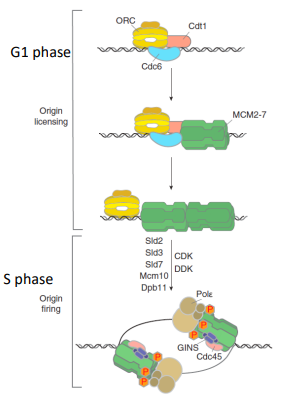
\includegraphics{../_resources/cf33180a017e8d51c049566410ac8b20.png}

There are many more licensed origins than the ones that are actually
used. Some are used early, some later, some never at all and are used as
backup if something goes wrong.
If an oncogene is to induce proliferation, it has to induce these steps.
MYC, but also RAS and MAP kinases promote proliferation (figure \ref{fig:origins}).

\begin{figure}[H]
\centering
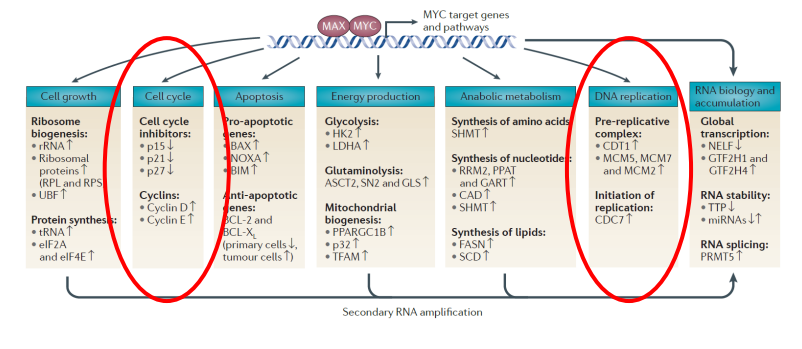
\includegraphics[width=0.5\textwidth]{../_resources/a78ad57bf8373a5417b0ddce30b8ed72.png}
\label{fig:origins}
\end{figure}
%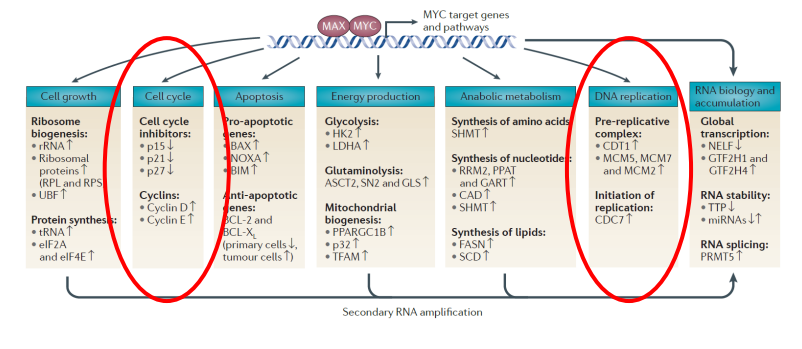
\includegraphics{../_resources/a78ad57bf8373a5417b0ddce30b8ed72.png}

Oncogene expression leads to transient upregulation of CDK6, and leads to altered replication timing. At the end, oncogenes all push the cell to enter phase S (figure \ref{fig:sphase}).

\begin{figure}[H]
\centering
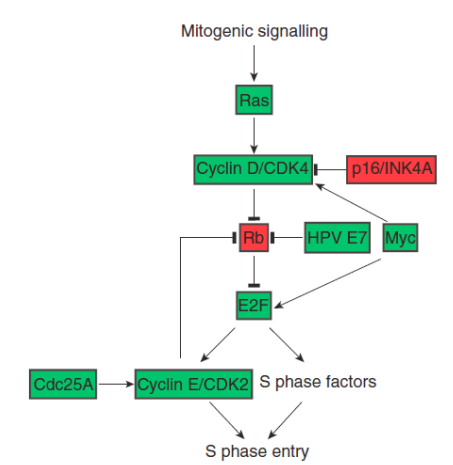
\includegraphics[width=0.4\textwidth]{../_resources/32b183547f544448275d6f43d7693d7e.png} 
\label{fig:sphase}
\end{figure}
%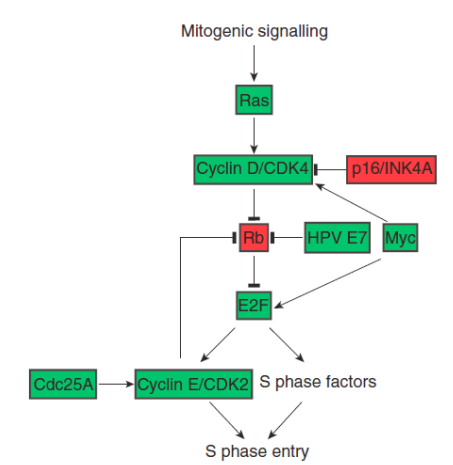
\includegraphics{../_resources/32b183547f544448275d6f43d7693d7e.png}

We end up with premature origin activation: maybe this is the reason why in
the previous FISH experiment we see many dots of replication, but
diploidy is maintained.

\textbf{Oncogene activation induces replication stress.} All the conditions in the first part of the picture (basically the premature of firing of all replicative factors, without the licensed origins, limited dNTPs) lead to some aberration to the chromosomes (figure \ref{fig:aber}).

\begin{figure}[H]
\centering
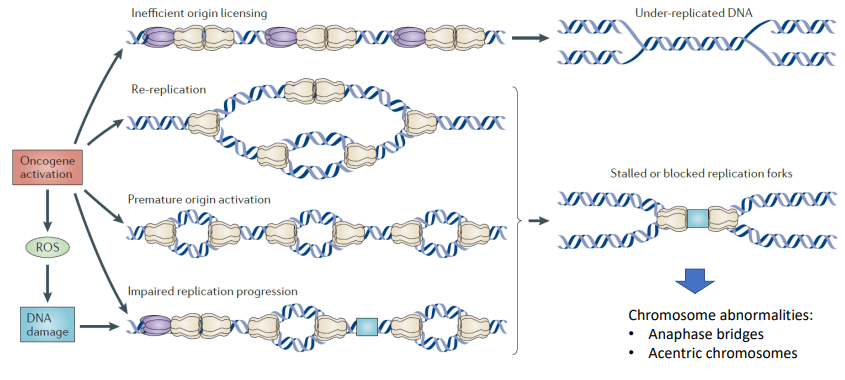
\includegraphics[width=0.6\textwidth]{../_resources/212276fa882f51c9df6ee225d31e5bae.png} 
\caption{Examples of chromosome abnormalities given by oncogene activation.}
\label{fig:aber}
\end{figure}
%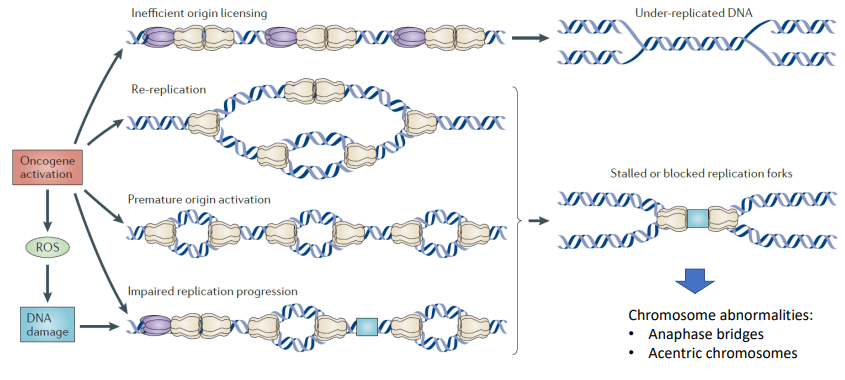
\includegraphics{../_resources/212276fa882f51c9df6ee225d31e5bae.png}

RPA binds to the lagging single strand left behind. 
ATR tries to fix the problem by blocking late origin firing and stabilizes (prevents collapse) of the replication fork. Also a DSB can recruit ATR (figure \ref{fig:bartkova}).

\begin{figure}[H]
\centering
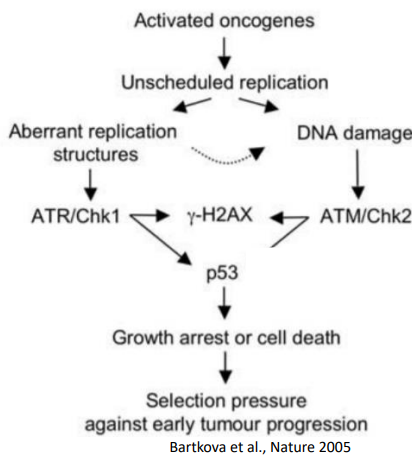
\includegraphics[width=0.4\textwidth]{../_resources/13c8849fd53903e2747fc9cc1a31fa57.png}  
\caption{Bartkova et al., Nature 2005}
\label{fig:bartkova}
\end{figure}
%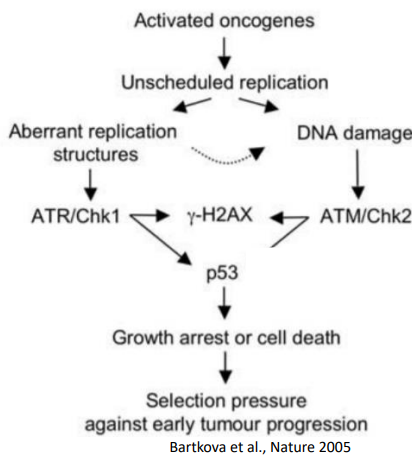
\includegraphics{../_resources/13c8849fd53903e2747fc9cc1a31fa57.png} 

We now have a system that wants to push to S phase, unleashing oncogenic
products.

\hypertarget{chromosome-abnormalities-due-to-pre-mitotic-defects-are-frequently-found-in-tumors}{%
\subsubsection{Chromosome abnormalities due to pre-mitotic defects are
frequently found in
tumors}\label{chromosome-abnormalities-due-to-pre-mitotic-defects-are-frequently-found-in-tumors}}

In pre-mitotic defects (the majority of the cases),  we will find acentric chromosomes or the presence of bridges (figure \ref{fig:defects}.

\begin{figure}[H]
\centering
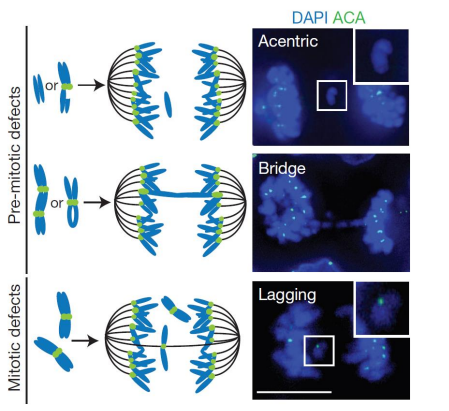
\includegraphics[width=0.5\textwidth]{../_resources/0a2601fb2d9e7056294ad4c26f178951.png}  
\label{fig:defects}
\end{figure}
%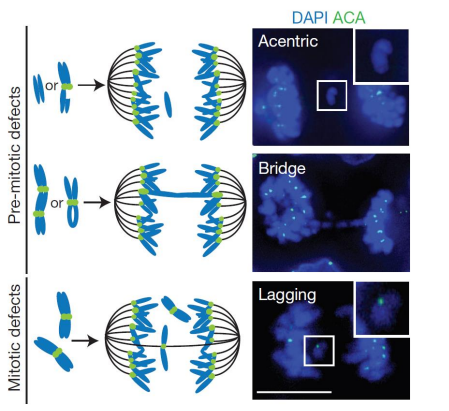
\includegraphics{../_resources/0a2601fb2d9e7056294ad4c26f178951.png}

Pharmacological induction of replication stress in HCT116 (CIN-) results
in \textbf{structural chromosome aberrations and segregation errors}.
Aphridicolin simulates stalled replication, by treating cells with no
defects we see the emergence of new defects, proving once again that
replication stress is the driving factor for DNA defects. Stress can be
found both in the chromosomes, but also at the end of the chromosomes.
However, nucleosides supplementation in CIN+ cell lines reduces DNA damage
and segregation error frequency.

A few key points: 
\begin{itemize}
\tightlist
\item Activated oncogenes cause replicative stress
characterized by increased numbers of stalled and collapsed replication
forks, accounting for early DNA damage
\item Under physiologic conditions,
DDR induced by stalled replication forks triggers a cell cycle arrest
and promotes replication fork restart or activation of dormant origins
of replication and DNA repair
\item Stalled replication forks induced by
activated oncogenes are not able to restart, due to the constitutive
insult. Under these conditions, the induced DDR triggers a persistent
state of growth arrest known as oncogeneinduced senescence
\item In the
early stages of cancer, replicative stress which may be able to promote
genome instability, induces a DNA damage response acting as an
anticancer barrier inducing senescence or apoptosis
\item When further
genetic or epigenetic changes down-regulate or impair the DDR signaling
(i.e ATM, ATR pathway) tumorigenesis can proceed
\end{itemize}

\hypertarget{transcription-replication-conflicts}{%
\subsubsection{Transcription replication
conflicts}\label{transcription-replication-conflicts}}

The problem is when oncogenes become aberrant: in normal situation we
need them to be functional.

\begin{figure}[H]
\centering
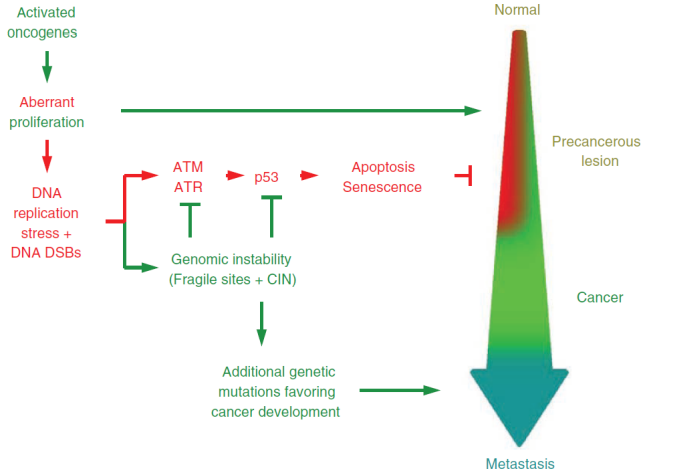
\includegraphics[width=0.5\textwidth]{../_resources/61c42671b1b95714d2335e1c23a75024.png} 
\label{fig:senescence}
\end{figure}
%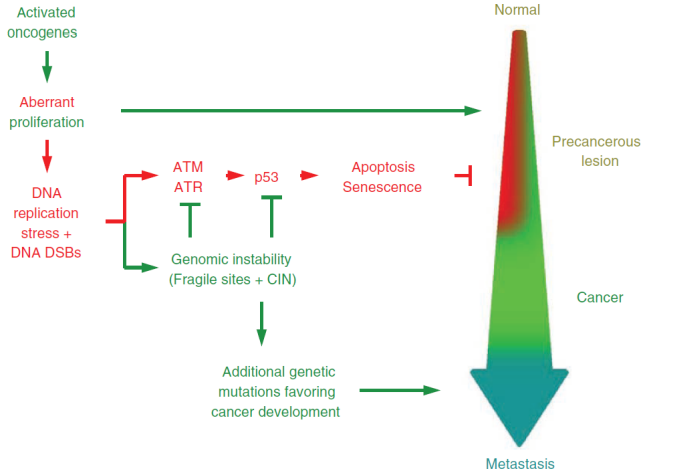
\includegraphics{../_resources/61c42671b1b95714d2335e1c23a75024.png}

Transcription is a natural obstacle to replication fork progression. In
aberrant replication, DNA will be broken in different sites. 
Transcription replication conflicts can induce replication stress
threatening genome stability and
occur head-on or co-directional. There's a reason why the OR is close to
the gene promoter:

\begin{figure}[h!]
\centering
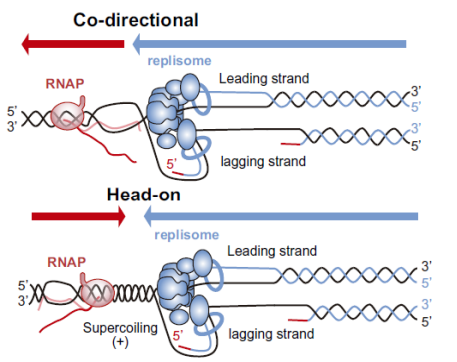
\includegraphics[width=0.5\textwidth]{../_resources/7e83b9f1b770e9e66657e633c833c9a4.png}
\label{fig:senescence}
\end{figure}
%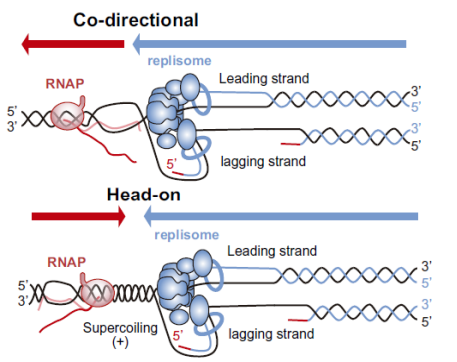
\includegraphics{../_resources/7e83b9f1b770e9e66657e633c833c9a4.png}

\begin{enumerate}
\def\labelenumi{\arabic{enumi}.}
\tightlist
\item
  HO stalling mechanisms:either conflict, generations of
  positive supercoiling (additional helicases needed to solve the coil)
  or RNAPolII is paused by G4.
\item
  In CD stalling mechanisms: no positive supercoiling building up
  (backtracking: RNAPollII moves back because the nucleotides are not
  properly base-paired, R-loop-induced Pausing).
\item
  CD restart mechanisms:

  \begin{enumerate}
  \def\labelenumii{\arabic{enumii}.}
  \tightlist
  \item
    Naked R-loop with some RNA primer on it (hybrid bypass)
  \item
    Same thing, but instead of bypassed by catpitalizing on the existing
    primer, the hybrid is unwound and resolved
  \item
    HO restart mechanisms

    \begin{enumerate}
    \def\labelenumiii{\arabic{enumiii}.}
    \tightlist
    \item
      the messiest is the presence of the superhelical, since it needs
      either homologous recombination or ligation through the use of other
      enzymes.
     
    \end{enumerate}
  \end{enumerate}
\end{enumerate}


\begin{figure}[H]
		\centering
 		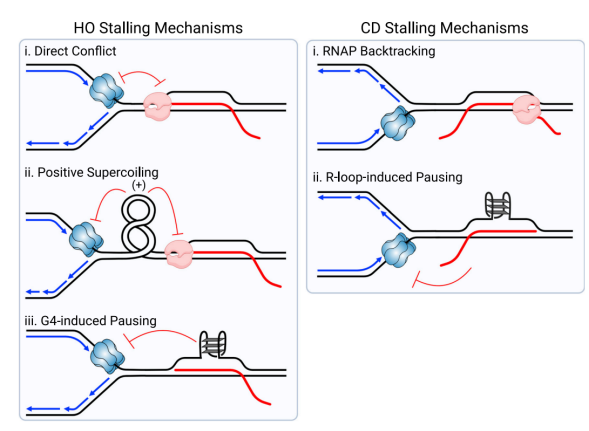
\includegraphics[scale = 0.4]{../_resources/78ecdeb0787ab87f0b7124de9a54c389.png}
        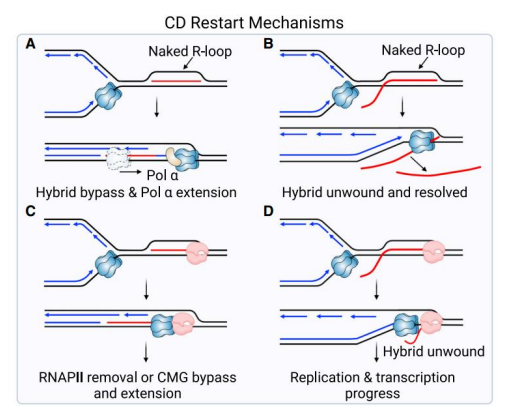
\includegraphics[scale = 0.4]{../_resources/5b8301b5dc4e4bdae69a035b325c110d.png}
        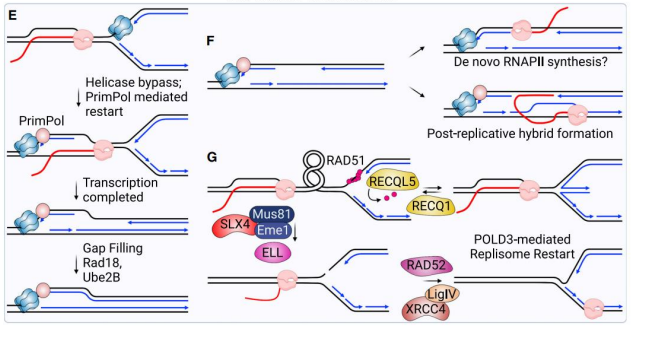
\includegraphics[scale = 0.4]{../_resources/7488f37079b01dd2811223bd1a82f7fb.png}
		\label{fig:senescence}
	\end{figure}
	
	
\textbf{Common fragile sites (CFS)} are loci prone to form breaks upon
replication stress and associate with recurrent rearrangements in
cancer. Indeed, there's evidence that oncogene-induced replication
stress preferentially targets common fragile sites in preneoplastic
lesions (figure \ref{fig:CFS}).

\begin{figure}
\centering
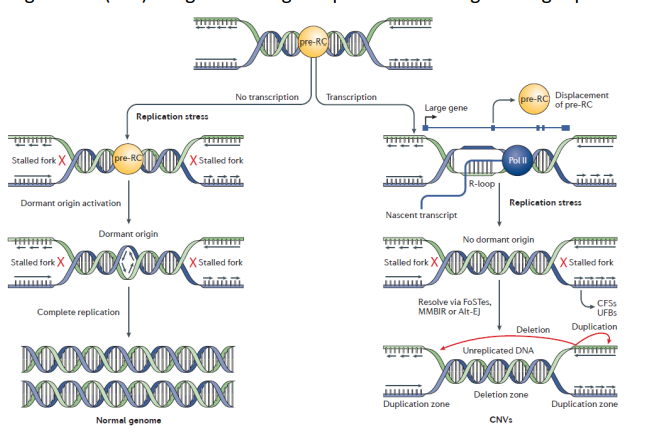
\includegraphics[width=0.5\textwidth]{../_resources/c0296c07042a0397b2b5c43d74b2f158.png}
\caption{Common fragile sites (CFS)}
\label{fig:CFS}
\end{figure}
%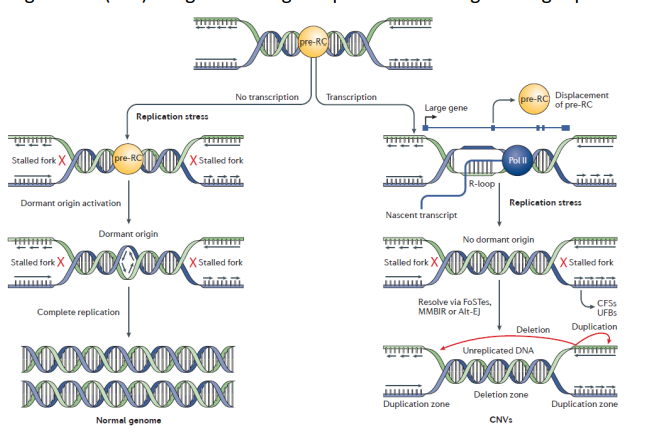
\includegraphics{../_resources/c0296c07042a0397b2b5c43d74b2f158.png}

\hypertarget{increased-global-transcription-activity-as-a-mechanism-of-replication-stress-in-cancer}{%
\subsubsection{Increased global transcription activity as a mechanism of
replication stress in
cancer}\label{increased-global-transcription-activity-as-a-mechanism-of-replication-stress-in-cancer}}

To study the increased activity, H-RAS is tracked, as its expression
associates with increased overall transcription. H-RAS expression also
associates with increased R-loops formation. Interestingly, \textbf{RAS
expression induces replication stress} (figure \ref{fig:RAS}).

\begin{figure}[h!]
\centering
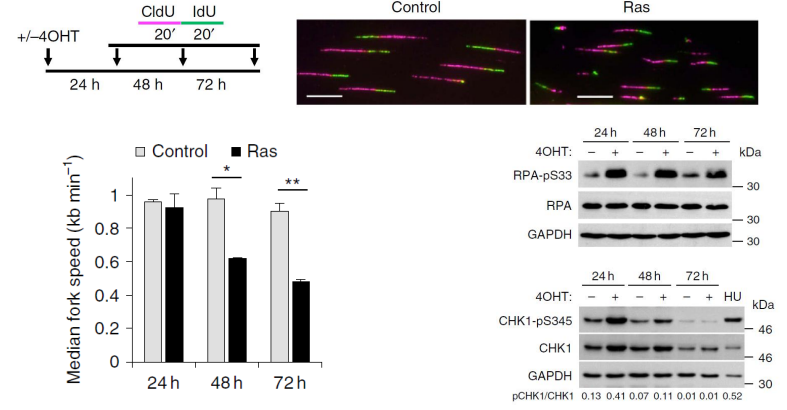
\includegraphics[width=0.5\textwidth]{../_resources/74f971d93ec73bb49f66e1c9f6c16c26.png}
\caption{RAS expression induces replication stress}
\label{fig:RAS}
\end{figure}
%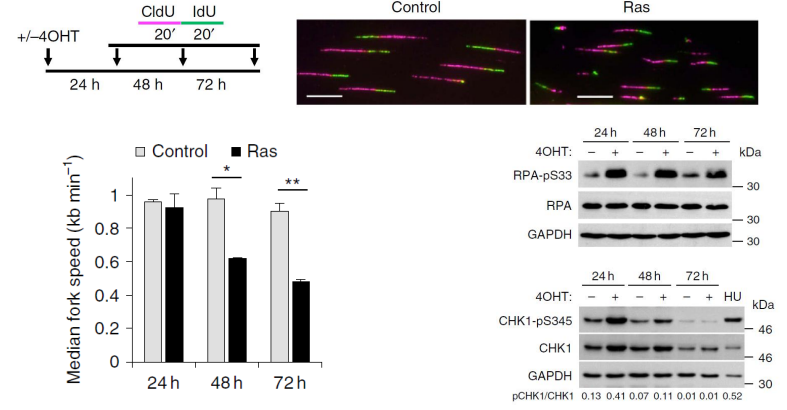
\includegraphics{../_resources/74f971d93ec73bb49f66e1c9f6c16c26.png}

Transcription inhibitor is added to the system, then the replication is
partially rescued $\rightarrow$ RAS-induced replication stress is
promoted by ongoing transcription. In the paper they also proposed a
model based on the fact that TBP is induces by RAS singalling. More TBP
$\rightarrow$ more promoters activated. Its depletion decreases the
production of mRNA. Increased transcription activity is a mechanism
contributing to (a more direct) replication stress in cancer.

\begin{figure}[H]
\centering
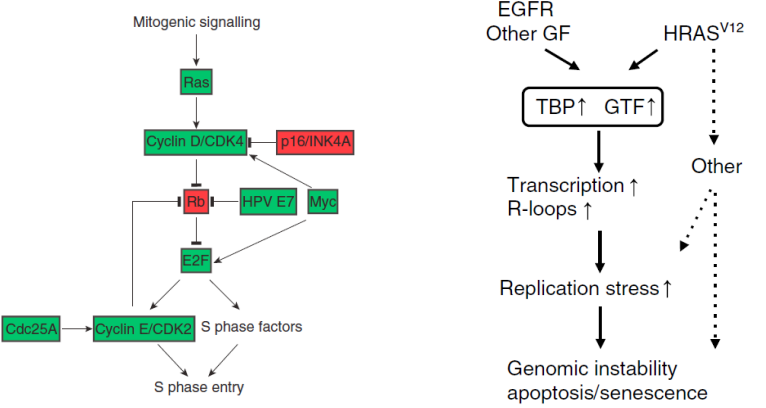
\includegraphics[width=0.5\textwidth]{../_resources/44bcc98a5cf90e0a6c62c0c54ac18ec8.png}
\label{fig:senescence}
\end{figure}
%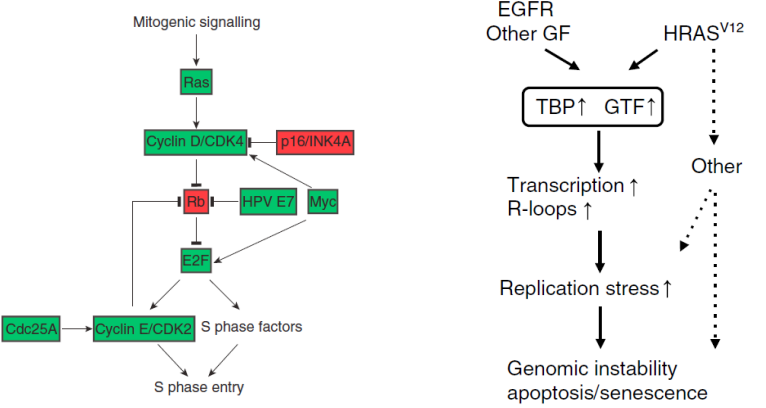
\includegraphics{../_resources/44bcc98a5cf90e0a6c62c0c54ac18ec8.png}

\begin{figure}[H]
\centering
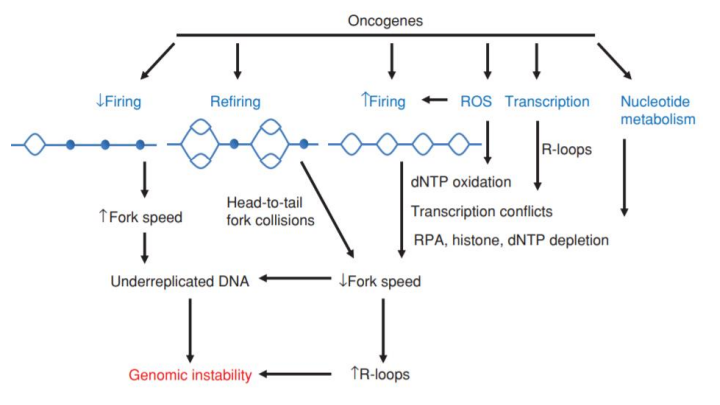
\includegraphics[width=0.5\textwidth]{../_resources/a522e1eccf4aff0b733df053f8ae4a38.png}
\caption{Oncogenes overview}
\end{figure}

\textbf{Main points:} 
\begin{itemize}
\tightlist
\item Oncogene expression/activation boosts
replication, transcription, R-loops formation leading to replicative
stress and activation of DDR 
\item DDR activation signals cell cycle block,
senescence or apoptosis, acting as tumor suppressor pathway
\item Impaired
DNA repair mechanisms allow accumulation of mutations
\item If mutations in
DDR pathways occur cells can bypass replicative stress, continuing
proliferating despite accumulating DNA lesions with consequent genome
instability
\end{itemize}


The source of activation of DDR pathway is replicative stress i.e.~dysregulation of replication machinery and involvement of transcription, which can collide with DNA replication processes, in particular when R-loops are present. Cells need to react quickly to this source of instability, as DNA damage can lead to single or double DNA breakage.

Until recently, only proteins were presumed to be involved in this signalling cascade.

In Figure \ref{fig:hnf} we visualize human normal fibroblasts (HNF) hit by an ionizing radiation - reproducing X-ray diagnostic procedure. This leads to DNA break and activation of DDR. The experiment was performed with siDICER (targeting and degrading dsDNA) $\rightarrow$ impaired activity apart from \(\gamma\)H2AX, which is phosphorylated quickly. siDROSHA also shows a similar pattern.

\begin{figure}
\centering
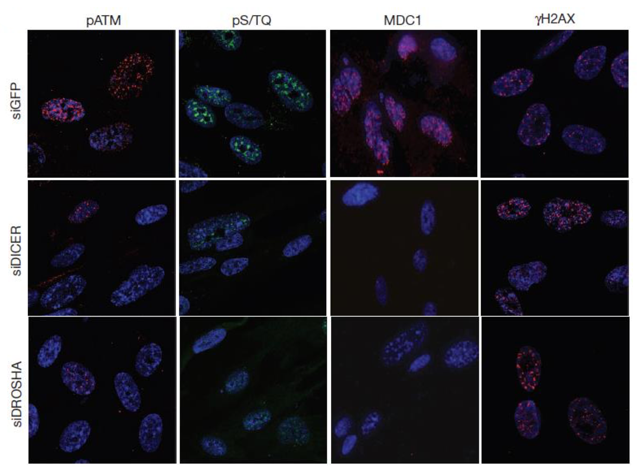
\includegraphics[width=0.5\textwidth]{Screen_Shot_2022-12-07_at_08-58-00.png}
\caption{Francia \emph{et al., Nature} 2012}
\label{fig:hnf}
\end{figure}

\hypertarget{biogenesis-of-canonical-mirna}{%
\section{Biogenesis of canonical miRNA}\label{biogenesis-of-canonical-mirna}}

These enzymes are involved in the maturation process of miRNAs. The pri-miRNA is shaped in a loop structure, DROSHA binds and then pre-miRNA is bound to exportin for the export in the cytoplasm. Once outside, DICER recognizes the stem loop and cuts RNA right at the loop to obtain a 20-25 nt sequence.

DICER and DROSHA inactivation impairs DDR loci formation in irradiated cells. The same occurs in mutant DICER (DICERexon5) DDR positive cells.

RFP 5' UTR for endogenously expressed RNA. Under normal condition the fluorescence is not seen (Figure \ref{fig:si}); if we keep the cells under the X-ray, we observe miR126 staining. If DICER is depleted, siDICER will exhibit increased signal. No 53BP1 is observed as the pathway is impaired. Lastly, they deplete proteins involved in transcription inhibition. 53BP1 is detected if cells are irradiated.

\begin{figure}
\centering
\includegraphics[width=0.5\textwidth]{Screen_Shot_2022-12-07_at_08-59-12.png}
\caption{Francia \emph{et al., Nature} 2012}
\label{fig:si}
\end{figure}

This suggests that the effect of DICER and DROSHA is independent from the canonical miRNA-mediated translational repression mechanisms. The knockdown impairs G1/S checkpoint; OIS (oncogene induced senescence) cells further supports that these enzymes are important for DDR.

\hypertarget{dicer-and-drosh-regulation-of-ddr-and-checkpoint-enforcement}{%
\section{DICER and DROSHA regulation of DDR and checkpoint enforcement}\label{dicer-and-drosh-regulation-of-ddr-and-checkpoint-enforcement}}

Cells treated with mild detergent promoting permeabilization of the membrane; add RNAse to degrade RNAs, marker of DDR will not be detected. When irradiating cells, this leads to DDR inhibition. If before fixing cells we introduce RNA after degradation, this enables the rescue of the effect. DDR activation is controlled by small RNA species of 20-35 nt.

Since irradiation leads to ds break in a random fashion, to gain more insight in the nature of RNAs and in the nature of the breaks they used NIH 2/4 cells, which have a construct containing Lac repeats and IScell1 restriction enzyme binding site. (Figure \ref{fig:lac}).  IS1 cuts 18 nt binding sites - the binding site does not contain this site. A DDR focus generated on a defined DSB can disassemble and reassemble in an RNA-dependent manner.

Site-specific DDR focus formation is RNase A sensitive. Only RNA from the cut NIH2/4 cells can reassemble DDR focus formation. Is the RNA generated from the LacO-SceI cassette upon cut responsible to DDR foci formation?

\begin{figure}
\centering
\includegraphics[width=0.5\textwidth]{Screen_Shot_2022-12-07_at_09-03-41.png}
\caption{Francia \emph{et al., Nature} 2012}
\label{fig:lac}
\end{figure}

Deep-sequencing of libraries generated from short \textless200 nucleotides nuclear RNAs revealed short transcripts arising from the exogenous locus (LacO-Scel cassette).

Chemically synthesized small RNAs are sufficient to restore DDR focus formation in RNase A-treated cells in a sequence-specific manner.

\hypertarget{ddrnas}{%
\section{DDRNAs}\label{ddrnas}}

DDRNAs are DICER- and DROSHA-dependent products with the sequence of the damaged site. DDRNAs act differently from canonical miRNAs. For instance, microinjected DDRNAs (with complementary sequence to I-Scel binding site) localize to the DNA damage site. Lac+Tet are used as are repetitive elements, but in principle any sequence is fine.

Sequence-specific localization of DDRNAs at DNA damage sites is functional and transcription-dependent. The RNAs co-localize by the ds-breaks complementary to their sequence and manage to do so even in the absence of DROSHA and DICER $\rightarrow$ transcription-dependent manner, PolII transcription at DSBs is required for DDRNAs localization to DSBs and DDR foci formation (Figure \ref{fig:dd1}).

\begin{figure}
\centering
\includegraphics[width=0.5\textwidth]{Screen_Shot_2022-12-07_at_09-15-58.png}
\caption{Michelini \emph{et al., Nature Cell Biology} 2017}
\label{fig:dd1}
\end{figure}

DDRNAs localize to their homologous damaged site where they stimulate DDR focus formation in an RNA polII-dependent manner.

The investigation of transcription around DSB by RNA-FISH and RT-qPCR analysis allows us to understand the direction in which transcription is occurring. Once there is a cut, mainly \emph{from} (outward) transcripts are visualized, but also some \emph{to} (inward) transcript. (Figure \ref{fig:dd2}).

\begin{figure}
\centering
\includegraphics[width=0.5\textwidth]{Screen_Shot_2022-12-07_at_09-23-19.png}
\caption{Michelini \emph{et al., Nature Cell Biology} 2017}
\label{fig:dd2}
\end{figure}

dilncRNAs (damage induced lncRNAs) are transcribed by polII from DSBs, localize at DSBs where they are processed by DROSHA and DICER to generate DDRNAs. dilncRNA and DDRNAs induction are early DSB signals that together with \(\gamma\)H2AX may nucleate DDR focus formation.

ChIP revealed that RNAPII, RNAPII pSer5 and RNAPII pSer2 are enriched at the DSB following cut induction. It was observed that the transcription starts exactly from the extremity of the DSB, somehow Pol II must find the exact site $\rightarrow$ we said that it must be recruited at the promoter, how is it activating transcription at this site?

The MRN complex might lead to the recruitment of RNA PolII. Indeed, the MRN complex binds to RNAPII following irradiation (DNA damage) and is necessary for RNAPII transcription at DSBs. RNAPII transcription is further necessary for DDR focus formation and DNA repair.

\hypertarget{ddrnas-and-dilncrnas-regulate-ddr-and-dna-repair}{%
\subsection{DDRNAs and dilncRNAs regulate DDR and DNA repair}\label{ddrnas-and-dilncrnas-regulate-ddr-and-dna-repair}}

53BP1 interacts with DDRNAs and dilncRNAs. DDRNAs and dilncRNAs might act as scaffolds and stabilizers of the complex in DDR and DNA repair.

\textbf{Antisense oligonucletide gene knock-down:} no phosphodiesteric bond, posphotionate bond. This chemistry allows a stabler interaction and avoids endogenous enzyme degradation. 

ASOs prevents dilncRNA--DDRNA interaction, which affects 53BP1 focus formation.

\begin{figure}
\centering
\includegraphics[width=0.5\textwidth]{Screen_Shot_2022-12-07_at_09-50-28.png}
\caption{Michelini \emph{et al., Nature Cell Biology} 2017}
\end{figure}

\begin{figure}
\centering
\includegraphics[width=0.4\textwidth]{Screen_Shot_2022-12-07_at_09-51-02.png}
\caption{Michelini \emph{et al., Nature Cell Biology} 2017}
\end{figure}

The extremities of DSBs act as transcriptional promoters regardless of the genomic location, through MRN-PolII interaction. Damage-induced transcription represents one of the earliest events following DSBs generation, together with \(\gamma\)HSAX. DSBs-induced transcription nucleates DDR foci formation at least in part due to DDRNAs-53BP1 interaction and is important to DSBs repair.

\hypertarget{rna-pol-ii-recruitment-at-dsbs}{%
\section{RNA Pol II recruitment at DSBs}\label{rna-pol-ii-recruitment-at-dsbs}}

ChIP shows that 2,000 bp or more downstream we do not have a signal from relevant TFs in RNAPolII recruitment.

Stochastic optical reconstruction microscopy (STORM) reveals colocalization between transcription effectors and \(\gamma\)H2AX in NCS treated cells. NCS is a drug promoting DNA breaks randomly.

Enrichment of the indicated transcription effectors and MRN at a site-specific DSB in the indicated HeLa Kd cells. Transcription repression by multiple means reduces DDR signaling.

\textbf{Main findings of the study}

\begin{itemize}
\tightlist
\item
  The MRN complex recognizes the extremities of DSBs and recruits the PIC, Mediator and CDK9 to promote RNA polII transcription
\item
  Inactivation of PIC and inhibition of transcription impair DDR signaling and repair
\item
  DSBs act as sites of sequence- and promoter- independent recruitment of the transcriptional machinery
\item
  The function of transcription in the DDR signaling is dependent on dilncRNA synthesis
\item
  \(\gamma\)H2AX acts as docking site for the recruitment of DDR factors at DSBs, dilncRNAs and DDRNAs can act in promoting and stabilizing these complexes at DSBs
\end{itemize}
